\documentclass[a4paper,11pt]{article}
\usepackage[utf8]{inputenc}
\usepackage[T1]{fontenc}
\usepackage[english]{babel}
\usepackage{tikz}
\usetikzlibrary{arrows.meta, positioning, shapes, backgrounds}
\usepackage{adjustbox}
\usepackage{geometry}
\geometry{margin=1.5cm}

\pagestyle{empty}

\begin{document}

% =====================
% GLOBAL TITLE
% =====================
\begin{center}
  \Large \textbf{Simplified Microservices Architecture -- DeepSeek}
\end{center}
\vspace{0.5cm}

% =====================
% GLOBAL DIAGRAM
% =====================
\begin{adjustbox}{max width=\textwidth, center}
\begin{tikzpicture}[
    component/.style={rectangle, draw=black, rounded corners, minimum width=2.6cm, minimum height=1cm, align=center, font=\footnotesize, fill=blue!10},
    infra/.style={rectangle, draw=black, minimum width=2.6cm, minimum height=1cm, align=center, font=\footnotesize, fill=gray!15},
    actor/.style={ellipse, draw=black, minimum width=2cm, minimum height=0.8cm, align=center, font=\footnotesize, fill=green!15},
    arrow/.style={-Latex, thick}
]

% ==== ACTORS ====
\node[actor] (web) {Web Client};
\node[actor, right=2cm of web] (mobile) {Mobile Client};

% ==== API Gateway ====
\node[component, below=1.8cm of $(web)!0.5!(mobile)$] (gateway) {API Gateway};

% ==== CORE SERVICES ====
\node[component, below=2cm of gateway] (inference) {Inference Service};
\node[component, left=3.2cm of inference] (user) {User Service};
\node[component, right=3.2cm of inference] (rag) {RAG Service};

% ==== SUPPORT ====
\node[component, below=2cm of inference, fill=orange!15] (monitor) {Monitoring \& Logs};

% ==== INFRASTRUCTURE ====
\node[infra, below=1.5cm of user] (db) {Database};
\node[infra, below=1cm of inference] (vector) {Vector Store};
\node[infra, below=1.5cm of rag] (storage) {File Storage};

% ==== CONNECTIONS ====
\draw[arrow] (web) -- (gateway);
\draw[arrow] (mobile) -- (gateway);

\draw[arrow] (gateway) -- (user);
\draw[arrow] (gateway) -- (inference);
\draw[arrow] (gateway) -- (rag);

\draw[arrow] (user) -- (db);
\draw[arrow] (inference) -- (vector);
\draw[arrow] (rag) -- (storage);

\draw[arrow, dashed] (user) -- (monitor);
\draw[arrow, dashed] (inference) -- (monitor);
\draw[arrow, dashed] (rag) -- (monitor);

% ==== LEGEND ====
\node[draw, fill=white, rounded corners, below=1.5cm of monitor, align=left, font=\scriptsize] (legend) {
  \textbf{Legend:}\\
  \begin{tabular}{@{}l@{\hspace{0.6em}}l@{}}
    \tikz\draw[fill=green!15, draw=black] (0,0) ellipse (0.35 and 0.25); & Client \\
    \tikz\draw[fill=blue!10, draw=black, rounded corners] (0,0) rectangle (0.45,0.3); & Microservice \\
    \tikz\draw[fill=orange!15, draw=black, rounded corners] (0,0) rectangle (0.45,0.3); & Support \\
    \tikz\draw[fill=gray!15, draw=black] (0,0) rectangle (0.45,0.3); & Infrastructure \\
    \tikz{\draw[arrow] (0,0) -- (0.5,0);} & Communication \\
    \tikz{\draw[arrow, dashed] (0,0) -- (0.5,0);} & Monitoring
  \end{tabular}
};

\end{tikzpicture}
\end{adjustbox}

% =====================
% API GATEWAY ANALYSIS
% =====================
\newpage
\section{API Gateway Analysis}

\subsection*{Role and Definition}
The API Gateway acts as a single entry point for clients.  
It centralizes access to microservices and ensures critical functions such as routing, security, and data aggregation.

\subsection*{Main Responsibilities}
\begin{itemize}
    \item Request routing to microservices.
    \item Aggregation of responses from multiple services.
    \item Authentication and authorization (OAuth2, JWT).
    \item Protocol transformation (REST, gRPC, WebSocket).
    \item Metrics and logs collection for monitoring.
    \item Rate limiting and throttling.
\end{itemize}

\subsection*{Advantages}
\begin{itemize}
    \item Simplifies client access with a single entry point.
    \item Centralizes security and global policies.
    \item Supports response aggregation and improves performance.
    \item Facilitates scalability and modularity.
\end{itemize}

\subsection*{Limitations}
\begin{itemize}
    \item Risk of \textbf{Single Point of Failure}.
    \item Additional latency.
    \item Complexity in configuration and maintenance.
\end{itemize}

% =====================
% UML DIAGRAM - API GATEWAY
% =====================
\begin{center}
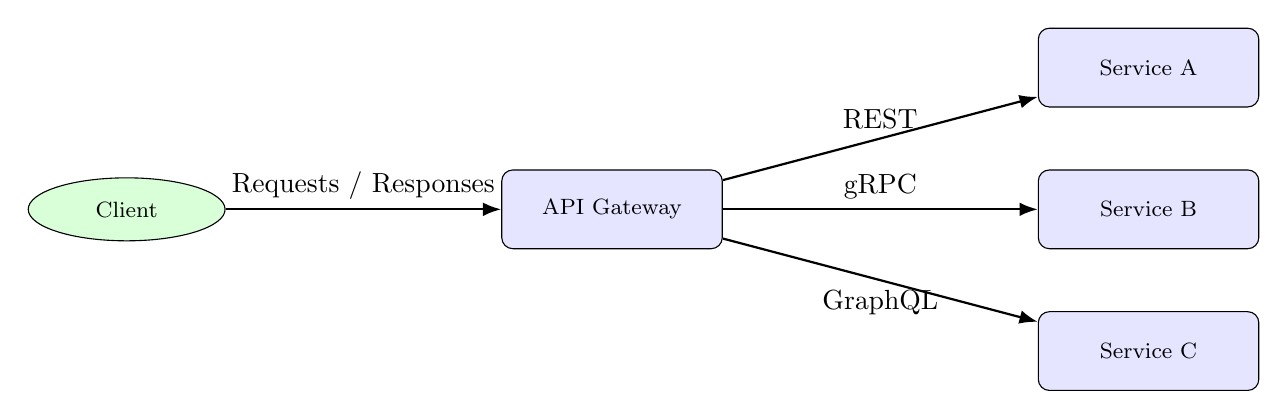
\begin{tikzpicture}[
    component/.style={rectangle, draw=black, rounded corners, minimum width=2.8cm, minimum height=1cm, align=center, font=\footnotesize, fill=blue!10},
    actor/.style={ellipse, draw=black, minimum width=2.5cm, minimum height=0.8cm, align=center, font=\footnotesize, fill=green!15},
    arrow/.style={-Latex, thick}
]

% ==== Client ====
\node[actor] (client) {Client};

% ==== API Gateway ====
\node[component, right=3.5cm of client] (apigw) {API Gateway};

% ==== Microservices ====
\node[component, right=4cm of apigw, yshift=1.8cm] (serviceA) {Service A};
\node[component, right=4cm of apigw] (serviceB) {Service B};
\node[component, right=4cm of apigw, yshift=-1.8cm] (serviceC) {Service C};

% ==== Relations ====
\draw[arrow] (client) -- (apigw) node[midway, above]{Requests / Responses};
\draw[arrow] (apigw) -- (serviceA) node[midway, above]{REST};
\draw[arrow] (apigw) -- (serviceB) node[midway, above]{gRPC};
\draw[arrow] (apigw) -- (serviceC) node[midway, below]{GraphQL};

\end{tikzpicture}
\end{center}

\captionof{figure}{UML diagram of the API Gateway and its interactions.}


\section{\textbf{Internal Architecture of the API Gateway}} 

\vspace{0.5cm}

\begin{center}
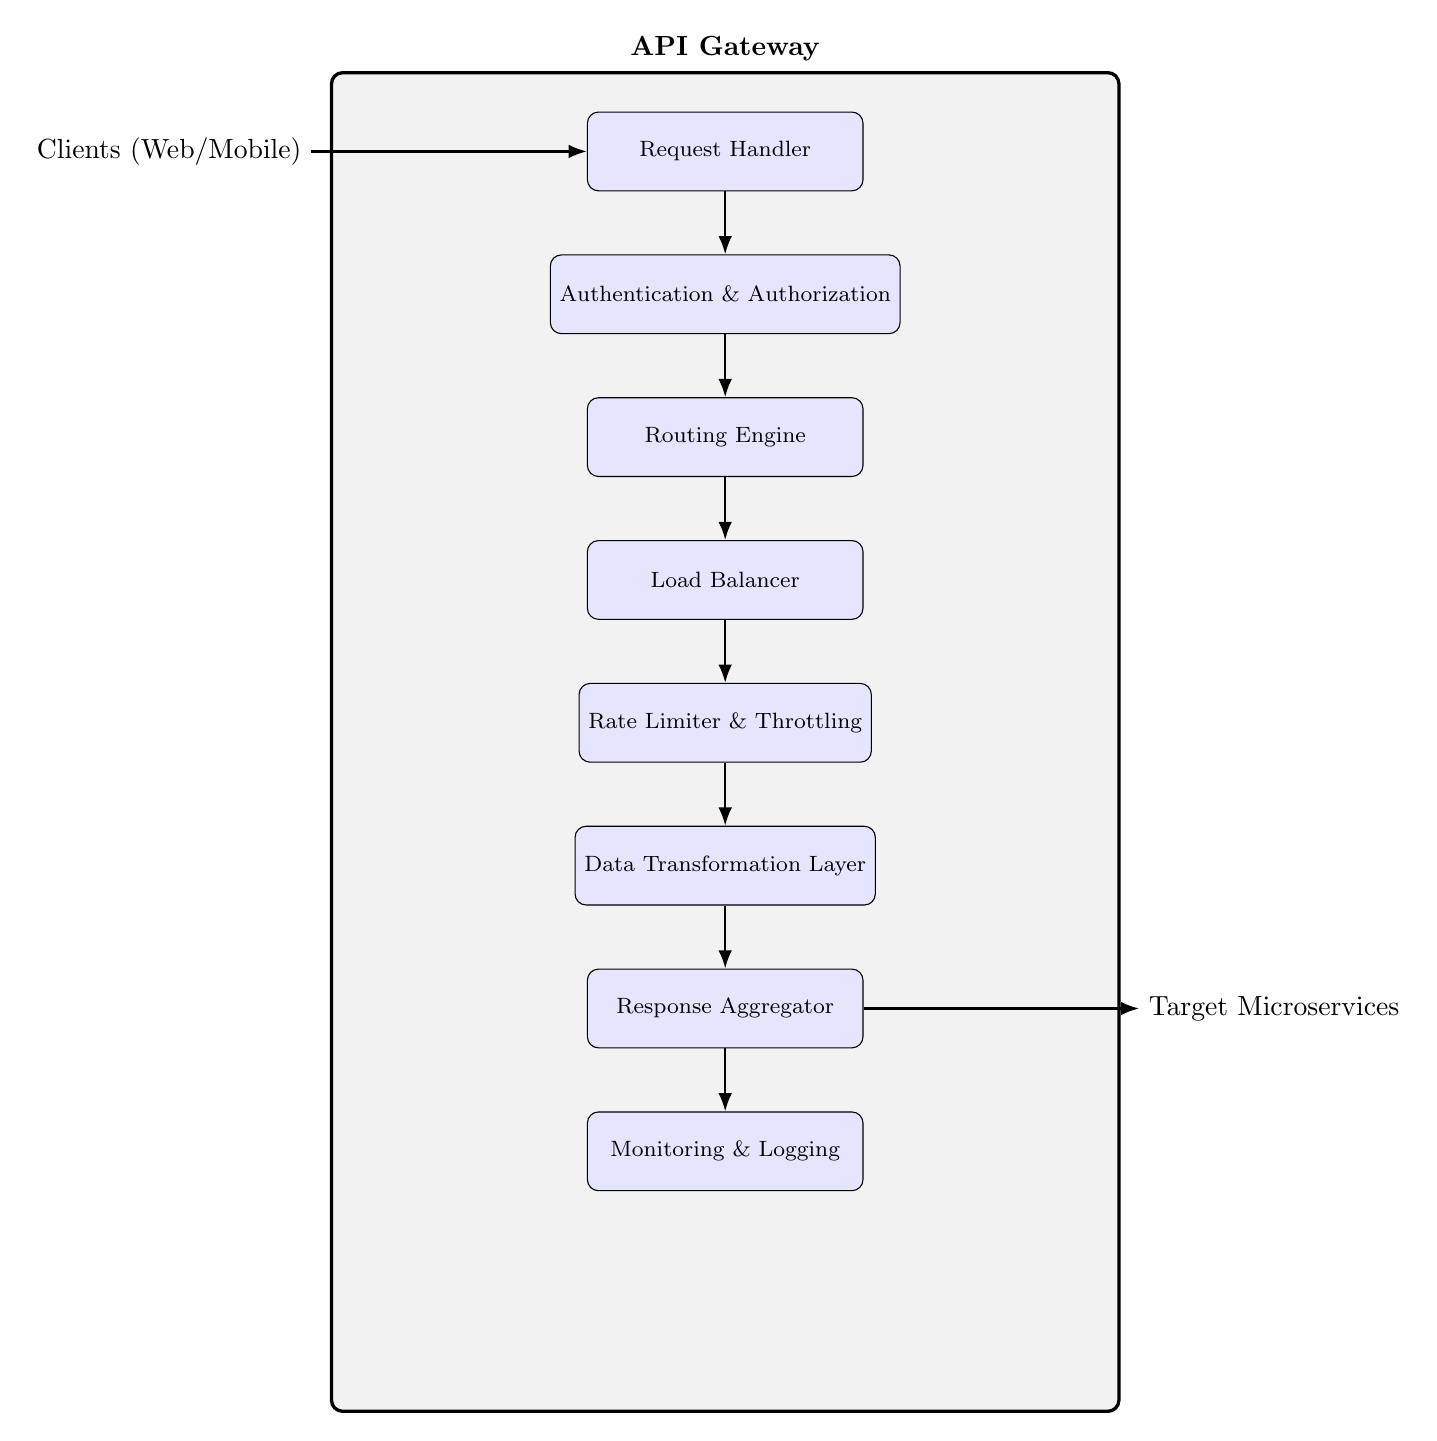
\begin{tikzpicture}[
    component/.style={rectangle, draw=black, rounded corners, minimum width=3.5cm, minimum height=1cm, align=center, font=\footnotesize, fill=blue!10},
    arrow/.style={-Latex, thick}
]

% ==== API Gateway container ====
\node[rectangle, draw=black, very thick, rounded corners, minimum width=10cm, minimum height=17cm, label={[yshift=0cm]above:\textbf{API Gateway}}, fill=gray!10] (gateway) {};

% ==== Internal components ====
\node[component, yshift=7.5cm] (reqhandler) {Request Handler};
\node[component, below=0.8cm of reqhandler] (auth) {Authentication \& Authorization};
\node[component, below=0.8cm of auth] (routing) {Routing Engine};
\node[component, below=0.8cm of routing] (loadbal) {Load Balancer};
\node[component, below=0.8cm of loadbal] (ratelimit) {Rate Limiter \& Throttling};
\node[component, below=0.8cm of ratelimit] (transform) {Data Transformation Layer};
\node[component, below=0.8cm of transform] (aggregator) {Response Aggregator};
\node[component, below=0.8cm of aggregator] (monitor) {Monitoring \& Logging};

% ==== Arrows (internal flow) ====
\draw[arrow] (reqhandler) -- (auth);
\draw[arrow] (auth) -- (routing);
\draw[arrow] (routing) -- (loadbal);
\draw[arrow] (loadbal) -- (ratelimit);
\draw[arrow] (ratelimit) -- (transform);
\draw[arrow] (transform) -- (aggregator);
\draw[arrow] (aggregator) -- (monitor);

% ==== External labels ====
\node[left=3.5cm of reqhandler] (client) {Clients (Web/Mobile)};
\draw[arrow] (client) -- (reqhandler);

\node[right=3.5cm of aggregator] (services) {Target Microservices};
\draw[arrow] (aggregator) -- (services);

\end{tikzpicture}
\end{center}

% ------------------------
% Detailed Analysis : API Gateway
% ------------------------
\section{Detailed Analysis — Internal Architecture of the API Gateway}

\subsection{Objectives and Requirements}
The API Gateway plays a central role in controlling and orchestrating client access to DeepSeek's microservices.  

\textbf{Functional Objectives}:
\begin{itemize}
  \item Provide a unified and stable entry point for all clients (Web, Mobile, Third-party APIs).
  \item Authenticate and authorize requests.
  \item Route requests to the appropriate services and aggregate responses when necessary.
  \item Perform protocol and data format transformations (REST $\leftrightarrow$ gRPC, JSON, GraphQL).
  \item Enforce policies (rate limiting, quotas, canary routing).
\end{itemize}

\textbf{Non-Functional Requirements}:
\begin{itemize}
  \item High availability (replicas, multi-zone deployment).
  \item Low latency and ability to handle traffic spikes.
  \item Observability (metrics, logs, traces).
  \item Security (TLS, validation, WAF).
  \item Easy configuration and policy enforcement.
\end{itemize}

\subsection{Internal Components — Detailed Description}
\begin{description}
  \item[Request Handler] : entry point receiving HTTP/WS requests, extracting headers, body, correlation IDs; performs syntactic validations (size, JSON schema) and applies basic protections (payload limits).
  \item[Authentication \& Authorization] : verifies JWT/OAuth2 (signature via JWKS) or opaque tokens (introspection with an Auth Service). Enforces scope/role checks (RBAC/ABAC).
  \item[Rate Limiter \& Throttling] : applies quotas per key (IP, API key, userId). Common implementations: token-bucket or leaky-bucket, atomic counters in Redis (Lua scripts) for cluster safety.
  \item[Input Validation \& Sanitization] : schema validation, header sanitization, normalization (unicode, trim), injection protection.
  \item[Routing Engine / Service Discovery] : maps requests (path, host, header) to target services. Integrates discovery (Consul / Kubernetes API) and routing rules (versions, canary, A/B testing).
  \item[Load Balancer / Upstream Manager] : selects upstream instance (RoundRobin, least-connections, weighted), manages persistent connections (keep-alive), handles timeouts.
  \item[Circuit Breaker \& Retry Policy] : protects against degraded upstreams. Key parameters: failure threshold, time window, reset timeout, exponential backoff retry logic.
  \item[Protocol / Data Transformation] : converts REST $\leftrightarrow$ gRPC, shapes JSON, maps schemas, enriches responses, strips sensitive fields before sending.
  \item[Response Aggregator / Composer] : orchestrates parallel service calls, merges results, supports partial responses and fallback strategies.
  \item[Monitoring \& Logging] : exports structured logs, traces, and metrics (Prometheus, OpenTelemetry) for observability.
\end{description}

% =====================
% IMPROVEMENTS
% =====================
\section{Proposed Improvements for the API Gateway}

The \textbf{DeepSeek API Gateway} can be enhanced to improve security, performance, and governance.  
Key additions include:  

\begin{itemize}
  \item \textbf{Security:} WAF (Web Application Firewall), mTLS support, OAuth2 validation.
  \item \textbf{Performance:} distributed caching, intelligent load balancing, circuit breaker and retry logic.
  \item \textbf{Observability:} distributed tracing (OpenTelemetry), advanced monitoring, Prometheus metrics.
  \item \textbf{Flexibility:} multi-protocol support (REST, gRPC, GraphQL), data aggregation and advanced transformation.
  \item \textbf{Governance:} API schema validation (OpenAPI/JSON Schema), quotas, versioning, and service discovery.
\end{itemize}

\vspace{0.5cm}

\begin{center}
\Large \textbf{Enhanced Internal Architecture of the API Gateway}
\end{center}
\vspace{0.5cm}

\begin{adjustbox}{max width=\textwidth, center}
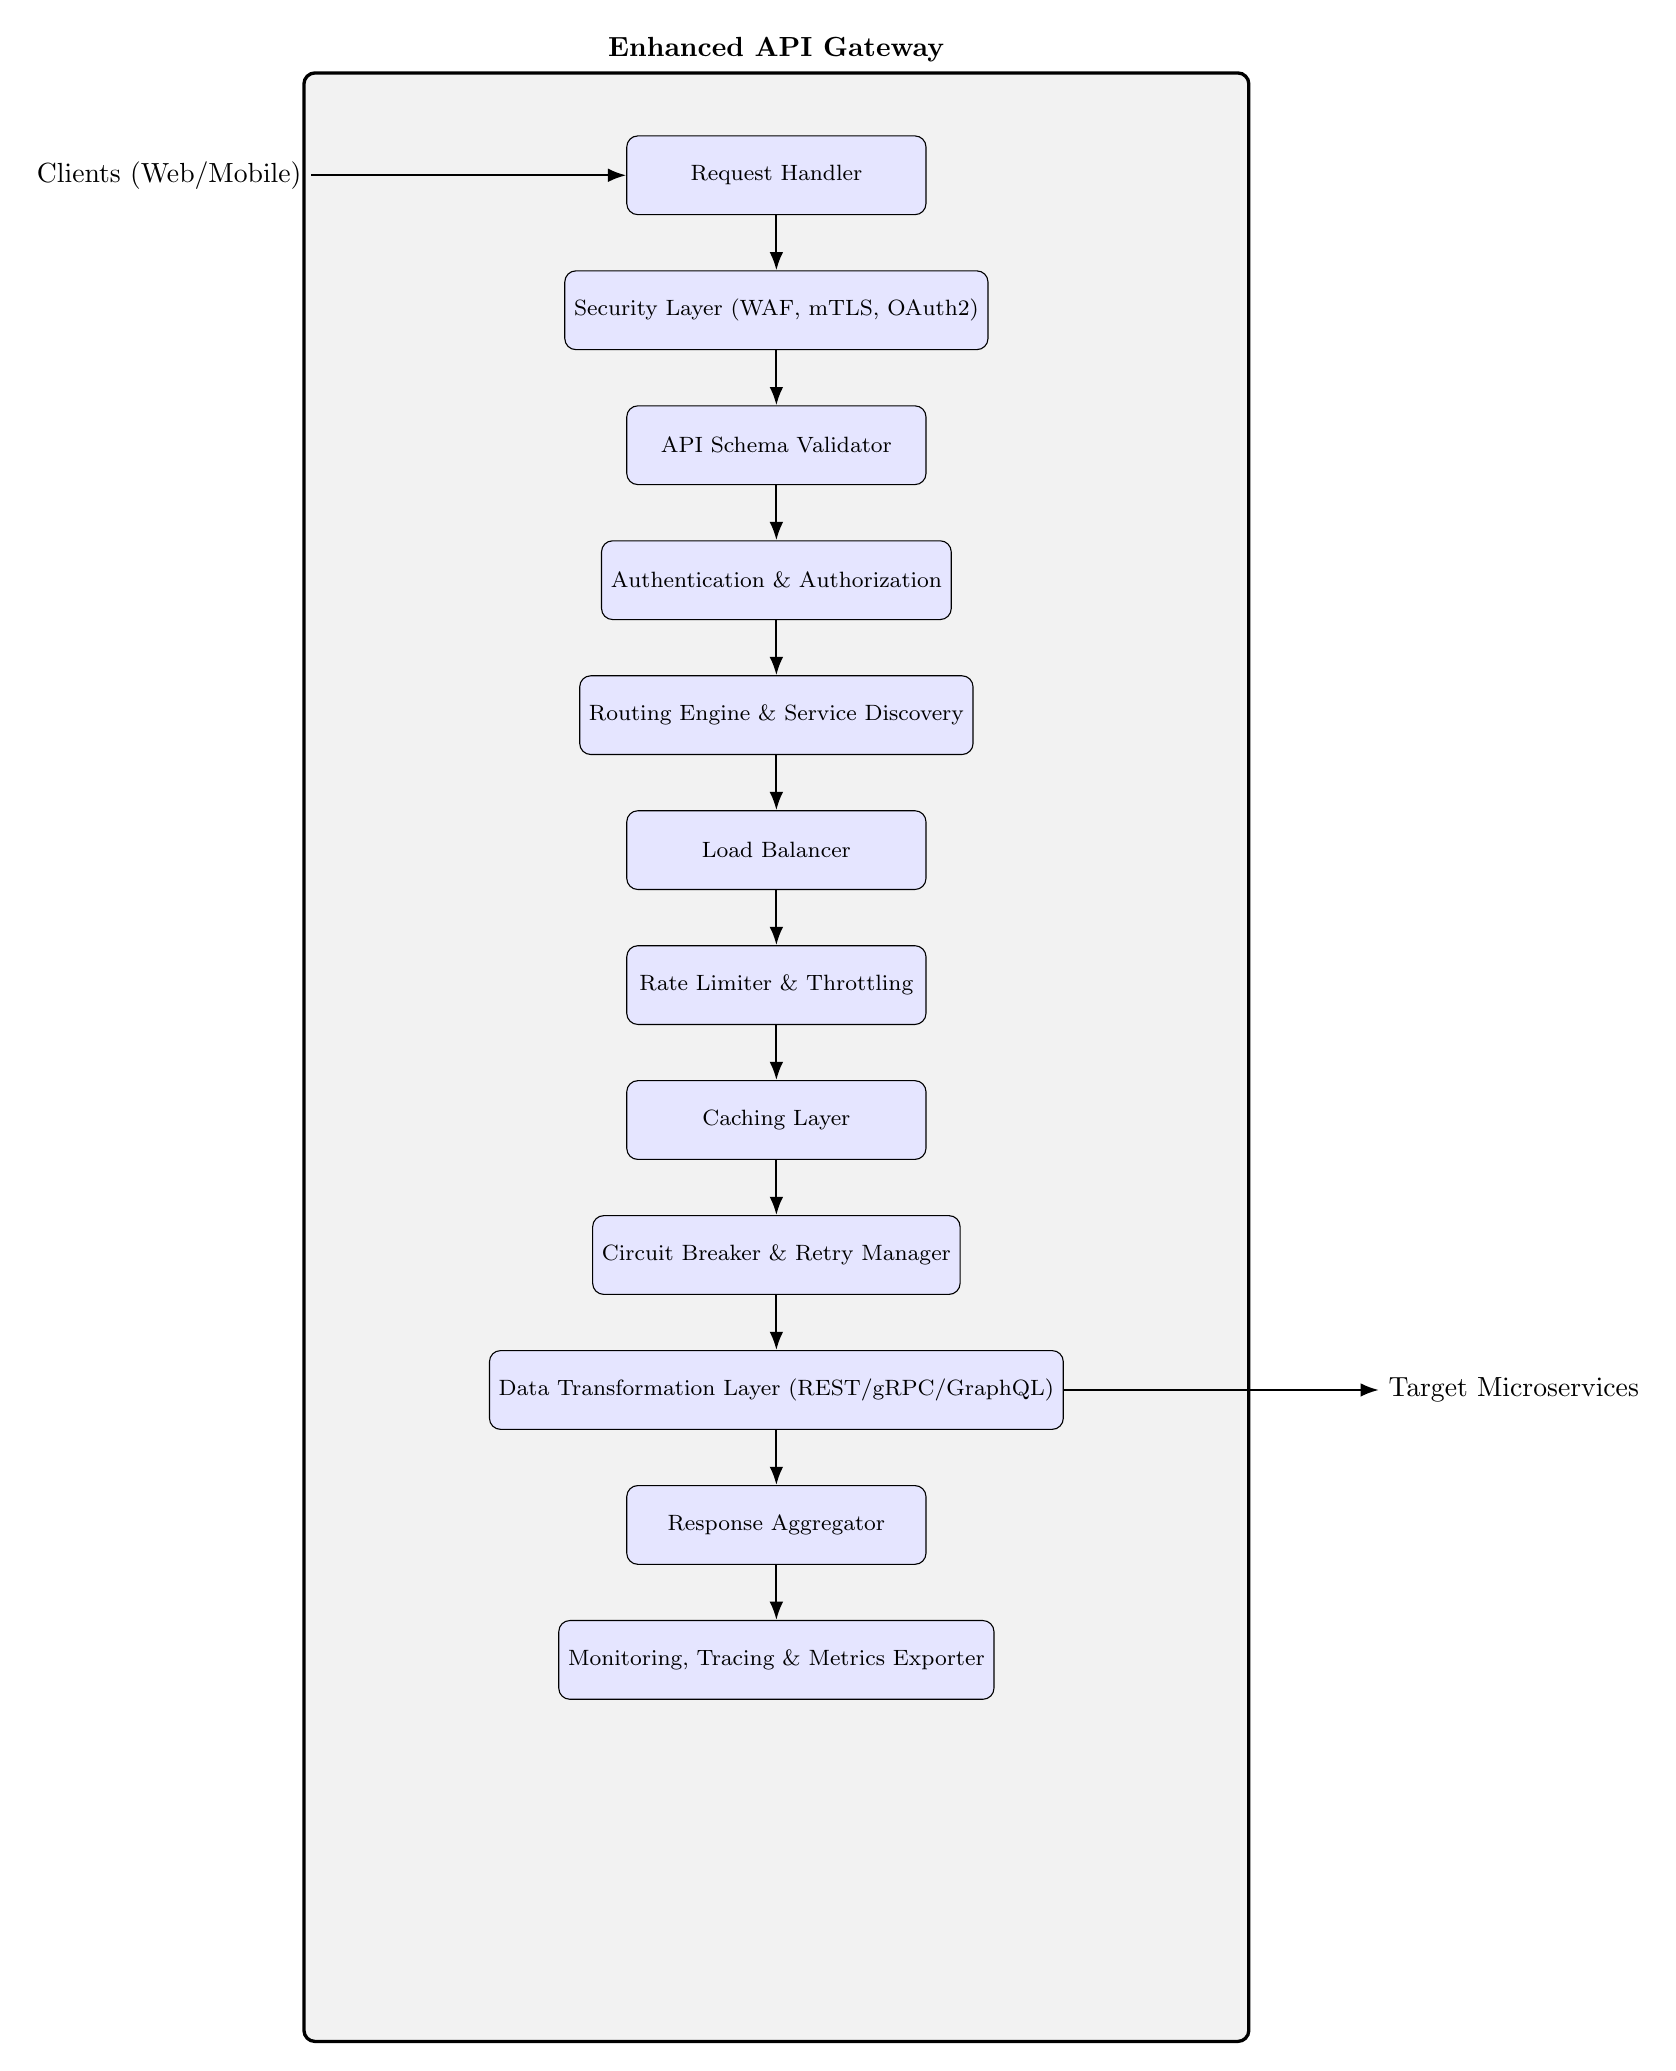
\begin{tikzpicture}[
    component/.style={rectangle, draw=black, rounded corners, minimum width=3.8cm, minimum height=1cm, align=center, font=\footnotesize, fill=blue!10},
    arrow/.style={-Latex, thick}
]

% ==== API Gateway container ====
\node[rectangle, draw=black, very thick, rounded corners, minimum width=12cm, minimum height=25cm, label={[yshift=0cm]above:\textbf{Enhanced API Gateway}}, fill=gray!10] (gateway) {};

% ==== Internal components ====
\node[component, yshift=11.2cm] (reqhandler) {Request Handler};
\node[component, below=0.7cm of reqhandler] (waf) {Security Layer (WAF, mTLS, OAuth2)};
\node[component, below=0.7cm of waf] (apivalid) {API Schema Validator};
\node[component, below=0.7cm of apivalid] (auth) {Authentication \& Authorization};
\node[component, below=0.7cm of auth] (routing) {Routing Engine \& Service Discovery};
\node[component, below=0.7cm of routing] (loadbal) {Load Balancer};
\node[component, below=0.7cm of loadbal] (ratelimit) {Rate Limiter \& Throttling};
\node[component, below=0.7cm of ratelimit] (cache) {Caching Layer};
\node[component, below=0.7cm of cache] (circuit) {Circuit Breaker \& Retry Manager};
\node[component, below=0.7cm of circuit] (transform) {Data Transformation Layer (REST/gRPC/GraphQL)};
\node[component, below=0.7cm of transform] (aggregator) {Response Aggregator};
\node[component, below=0.7cm of aggregator] (monitor) {Monitoring, Tracing \& Metrics Exporter};

% ==== Arrows (internal flow) ====
\draw[arrow] (reqhandler) -- (waf);
\draw[arrow] (waf) -- (apivalid);
\draw[arrow] (apivalid) -- (auth);
\draw[arrow] (auth) -- (routing);
\draw[arrow] (routing) -- (loadbal);
\draw[arrow] (loadbal) -- (ratelimit);
\draw[arrow] (ratelimit) -- (cache);
\draw[arrow] (cache) -- (circuit);
\draw[arrow] (circuit) -- (transform);
\draw[arrow] (transform) -- (aggregator);
\draw[arrow] (aggregator) -- (monitor);

% ==== External labels ====
\node[left=4cm of reqhandler] (client) {Clients (Web/Mobile)};
\draw[arrow] (client) -- (reqhandler);

\node[right=4cm of transform] (services) {Target Microservices};
\draw[arrow] (transform) -- (services);

\end{tikzpicture}
\end{adjustbox}

\section{\textbf{Client Request Execution Scenario - DeepSeek API Gateway}} 

\vspace{0.5cm}

\section*{Step-by-Step Scenario}

\begin{enumerate}
    \item \textbf{Client Request:} Web/Mobile client sends a request (REST/GraphQL) with JWT/OAuth2 token.
    \item \textbf{Request Handler:} Validates headers, payload, and assigns correlation ID.
    \item \textbf{Security Layer:} WAF blocks malicious patterns, mTLS ensures client identity, OAuth2 token validation.
    \item \textbf{API Schema Validator:} Validates request against OpenAPI/JSON Schema.
    \item \textbf{Authentication \& Authorization:} Checks RBAC/ABAC, denies unauthorized requests.
    \item \textbf{Routing Engine \& Service Discovery:} Maps request to appropriate microservices.
    \item \textbf{Load Balancer:} Selects upstream instances, manages connections and timeouts.
    \item \textbf{Rate Limiter \& Throttling:} Applies per-user/API key quotas.
    \item \textbf{Caching Layer:} Returns cached response if available, otherwise forwards request.
    \item \textbf{Circuit Breaker \& Retry:} Protects upstream services, retries failed calls, applies fallback if needed.
    \item \textbf{Data Transformation Layer:} Converts REST $\leftrightarrow$ gRPC/GraphQL, enriches request.
    \item \textbf{Microservice Calls:} Calls User, Inference, and RAG services in parallel.
    \item \textbf{Response Aggregator:} Combines results into a unified response, handles partial failures.
    \item \textbf{Monitoring \& Metrics:} Logs request/response, updates traces and metrics.
    \item \textbf{Client Response:} Sends aggregated response back to the client securely (TLS).
\end{enumerate}

\vspace{0.5cm}
\end{document}
